% ===================== PARTE 2: CORRECCIÓN (diapositivas 24-30) =====================
\parte{Corrección}{Corrección: ¿funciona sin romperse?}
  {Ser rápido no vale de nada si se rompe la memoria. Detectores automáticos, variantes rotas a propósito y la cota de intentos medida en el código real.}{s24}

\begin{frame}{Los detectores de errores dan lo mismo en las dos máquinas}
  \fuente{capturas/02, 03 y 09 (i5-10400) y resultados/david-ultra9-285/correccion (Ultra 9)}
  \footnotesize\renewcommand{\arraystretch}{1.15}
  \begin{tabularx}{\linewidth}{@{}p{0.29\linewidth}p{0.1\linewidth}XX@{}}
    \toprule
    \textbf{Prueba} & \textbf{Versión} & \textbf{Core i5-10400} & \textbf{Core Ultra 9 285}\\
    \midrule
    AddressSanitizer, 8 hilos & ingenua & \textcolor{rojo}{\emph{heap-use-after-free}} & \textcolor{rojo}{\emph{double-free}}\\
    AddressSanitizer, 8, 12 y 16 hilos & Autores & \textbf{0 errores} (53, 68 y 92\,ms) & \textbf{0 errores} (63, 98 y 137\,ms)\\
    ThreadSanitizer, 8 hilos & ingenua & \textcolor{rojo}{carreras de datos y \emph{heap-use-after-free}} & \textcolor{rojo}{carreras de datos y \emph{heap-use-after-free}}\\
    ThreadSanitizer, 8 y 16 hilos & Autores & \textbf{0 avisos} & \textbf{0 avisos}\\
    \bottomrule
  \end{tabularx}
  \vfill
  \begin{columns}[T]
    \column{0.49\textwidth}
    \porque{los dos detectores}{\textbf{ASan} marca cada bloque liberado y avisa si alguien lo vuelve a tocar. \textbf{TSan} registra quién accede a qué y avisa de dos accesos a la vez sin protección. Los dos solo ven lo que ocurre mientras miran.}
    \column{0.47\textwidth}
    \caja{La versión ingenua (leer el puntero y después sumar 1 al contador) cae en las dos máquinas, aunque con un síntoma distinto. La del paper no da ni un aviso, con hasta 16 hilos y 3,2 millones de operaciones.}
  \end{columns}
  \nota{s25}
\end{frame}

\begin{frame}{Romper el algoritmo a propósito: cada regla hace falta}
  \fuente{capturas/04 y 05 (i5-10400); resultados/david-ultra9-285/correccion/04 y 05 (Ultra 9); codigo/boceto/}
  \centering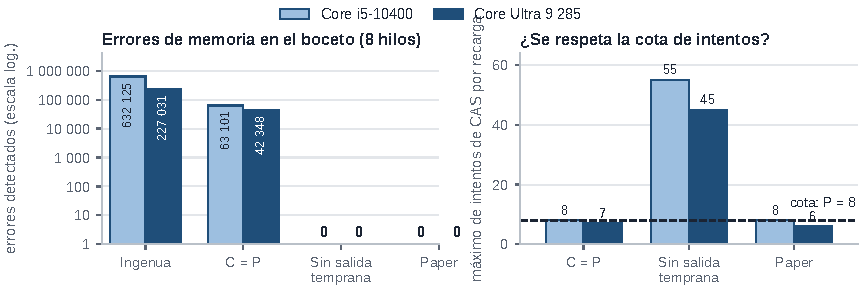
\includegraphics[width=\linewidth]{figuras/s26}
  \vfill\raggedright
  \caja{Sin la regla $C \ge 2P$ aparecen decenas de miles de errores. Sin la «salida temprana» no hay errores, pero los intentos pasan de 8 a 45-55: sigue siendo correcto, pero \textbf{ya no es wait-free}.}
  \nota{s26}
\end{frame}

\begin{frame}{La cota de intentos, medida en el código real de los autores}
  \fuente{resultados/david-ultra9-285/correccion/cota\_cas.csv (herramientas/correr\_cota\_cas.sh); EXPLICACION.md, Parte 6.5}
  \centering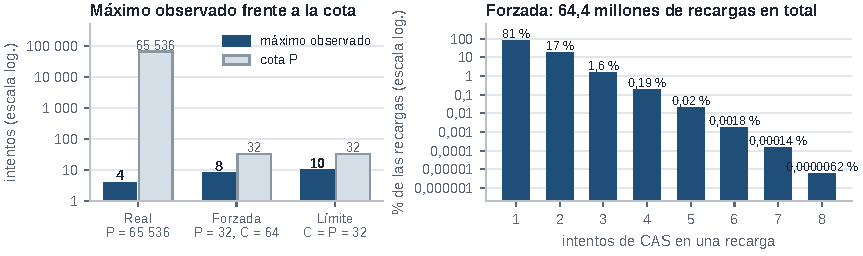
\includegraphics[width=\linewidth]{figuras/s27}
  \vfill\raggedright
  \begin{columns}[T]
    \column{0.49\textwidth}
    \caja{Con millones de recargas forzadas, el máximo fue \textbf{8 intentos frente a una cota de 32}. Con los valores reales, 4 frente a 65\,536.}
    \column{0.47\textwidth}
    \aviso{La fila «límite» viola R-1 ($C = P$): no falló porque había menos hilos que $P$, pero recarga en casi cada operación y rinde la mitad.}
  \end{columns}
  \nota{s27}
\end{frame}

\begin{frame}{La teoría que explica la cota}
  \fuente{de Wolff et al., secciones 4.1 y 4.2; EXPLICACION.md, Parte 3.6; capturas/08\_simulador.txt}
  \begin{columns}[T]
    \column{0.5\textwidth}
    \porque{la recarga termina}{%
      \begin{enumerate}\setlength{\itemsep}{2pt}
        \item El \texttt{load} es un \texttt{fetch\_sub} del peso: \textbf{nunca falla}.
        \item Si el peso cae bajo $P$, el hilo recarga con un CAS. Si el CAS falla, mira por qué:
          \begin{itemize}
            \item otro cambió el puntero o \textbf{ya recargó}: sale;
            \item el peso \textbf{bajó}: reintenta.
          \end{itemize}
        \item El peso empezó por debajo de $P$ y nunca baja de 0: como mucho \textbf{$P$ reintentos}.
        \item \textbf{R-1, $C \ge 2P$}: cada hilo solo puede gastar un vale de más antes de recargar, así que el peso nunca llega a ser negativo.
      \end{enumerate}}
    \column{0.46\textwidth}
    \sub{Simulador de intercalados}\footnotesize
    20\,000 ejecuciones por variante, comprobando las reglas tras cada paso atómico.
    \par\medskip
    \begin{tabularx}{\linewidth}{@{}Xr@{}}
      \toprule
      Variante & Ejecuciones con fallo\\
      \midrule
      \textbf{Algoritmo del paper} & \textbf{0}\\
      Ingenua & 4\,796\\
      Umbral 0 & 5\,089\\
      Sin reserva previa & 1\,171\\
      Sin salida temprana & 5\,467\\
      \bottomrule
    \end{tabularx}
    \par\medskip\scriptsize
    Con $P = 4$: 1 intento en el 80,1\,\% de las recargas, 2 en el 18,2\,\%, 3 en el 1,7\,\% y 4 en el 0,06\,\%. Nunca 5.
  \end{columns}
  \nota{s28}
\end{frame}

\begin{frame}{Los rivales tampoco rompen la memoria}
  \fuente{resultados/david-ultra9-285/correccion/10\_sanitizers\_rivales.txt (herramientas/sanitizers\_rivales.sh)}
  \footnotesize\renewcommand{\arraystretch}{1.15}
  \begin{tabularx}{\linewidth}{@{}p{0.38\linewidth}Xrr@{}}
    \toprule
    \textbf{Prueba} & \textbf{Algoritmos} & \textbf{Ejecuciones} & \textbf{Avisos}\\
    \midrule
    ASan + UBSan sobre \texttt{bench.cpp}, 8 y 16 hilos & Autores, Libstdc++, Williams, Mutex & 12 & \textbf{0}\\
    TSan sobre \texttt{bench.cpp}, 8 hilos & Autores, Libstdc++, Williams, Mutex & 4 & \textbf{0}\\
    ASan + UBSan sobre el \texttt{bench\_stack} oficial, 8 y 16 hilos, en Docker & Autores, Libstdc++, Williams, Folly, Anderson & 10 & \textbf{0}\\
    \bottomrule
  \end{tabularx}
  \vfill
  \begin{columns}[T]
    \column{0.49\textwidth}
    \caja{\textbf{Por qué importa:} si un rival ganara usando memoria ya liberada, su victoria no valdría. Ninguno de los seis lo hace en estas pruebas.}
    \column{0.47\textwidth}
    \aviso{Folly y Anderson no pasaron TSan: \texttt{libfolly.a} no está instrumentada y daría avisos falsos. Son 4 segundos por prueba y un solo escenario de contención fuerte ($n = 1$, $u = 50$\,\%).}
  \end{columns}
  \nota{s29}
\end{frame}

\begin{frame}{Lo que estas pruebas demuestran, y lo que no}
  \fuente{EXPLICACION.md, Parte 6.5 y Referencias}
  \begin{columns}[T]
    \column{0.48\textwidth}
    {\color{verde}\bfseries Lo que sí muestran}\par\smallskip
    \begin{itemize}\small
      \item Buscando el fallo con ganas, en dos máquinas y con tres herramientas, no apareció.
      \item Cada regla del diseño es necesaria: quitarla rompe la corrección o la cota.
      \item La cota se cumple con holgura en el código real: 8 frente a 32.
    \end{itemize}
    \column{0.48\textwidth}
    {\color{rojo}\bfseries Lo que no muestran}\par\smallskip
    \begin{itemize}\small
      \item Que el algoritmo sea correcto: una prueba nunca demuestra eso. La demostración está en el paper, secciones 4.1 y 4.2, y no se reproduce aquí.
      \item Que no haya errores en escenarios que no se probaron.
    \end{itemize}
  \end{columns}
  \vfill
  \caja{\textbf{Veredicto de las filas 14 y 15.} La recarga reintenta como mucho $P$ veces: \sirep. No hay \emph{use-after-free}, en lo probado: \sirep.}
  \nota{s30}
\end{frame}
